\documentclass[report.tex]{subfiles}

\begin{document}

\chapter{Applications to MCMC algorithms}
\label{chapter-bouncy-particle-sampler}



\begin{figure}
  \captionsetup{skip=0.75cm}
  \centering
  \begin{subfigure}{.25\textwidth}
    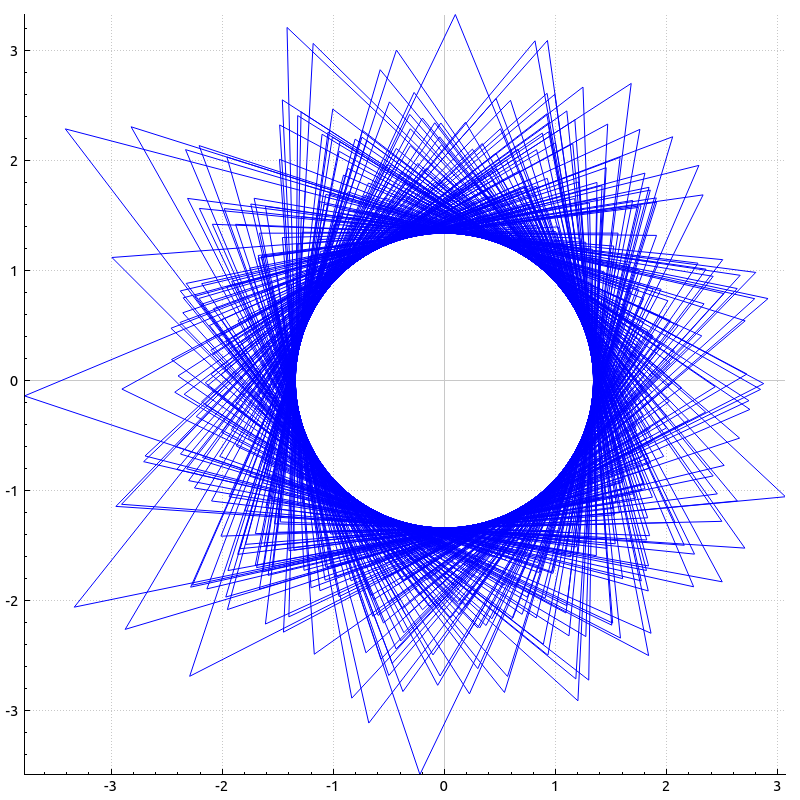
\includegraphics[width=\textwidth]{img/bps_ref_0_0001}
    \caption*{$\lambda_{\text{ref}} = 10^{-4}$}
  \end{subfigure}
  \begin{subfigure}{.25\textwidth}
    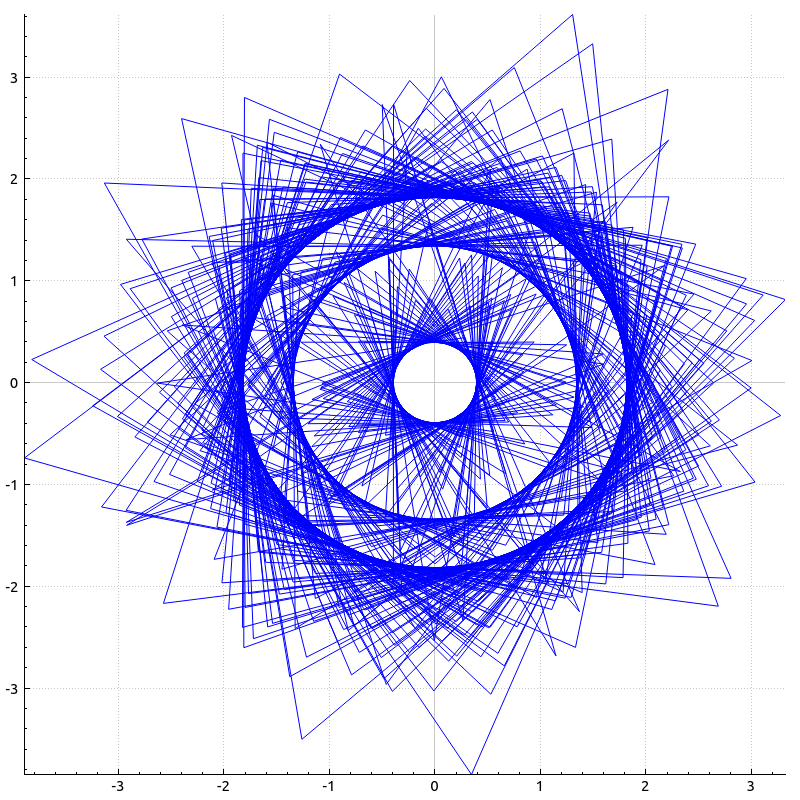
\includegraphics[width=\textwidth]{img/bps_ref_0_001}
    \caption*{$\lambda_{\text{ref}} = 10^{-3}$}
  \end{subfigure}
  \begin{subfigure}{.25\textwidth}
    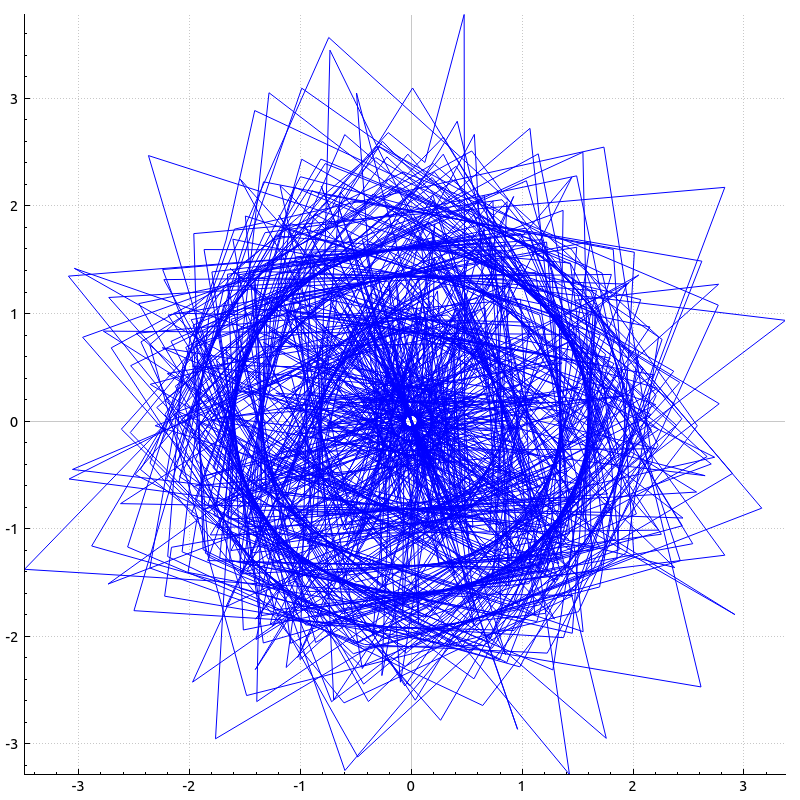
\includegraphics[width=\textwidth]{img/bps_ref_0_01}
    \caption*{$\lambda_{\text{ref}} = 10^{-2}$}
  \end{subfigure}
  \begin{subfigure}{.25\textwidth}
    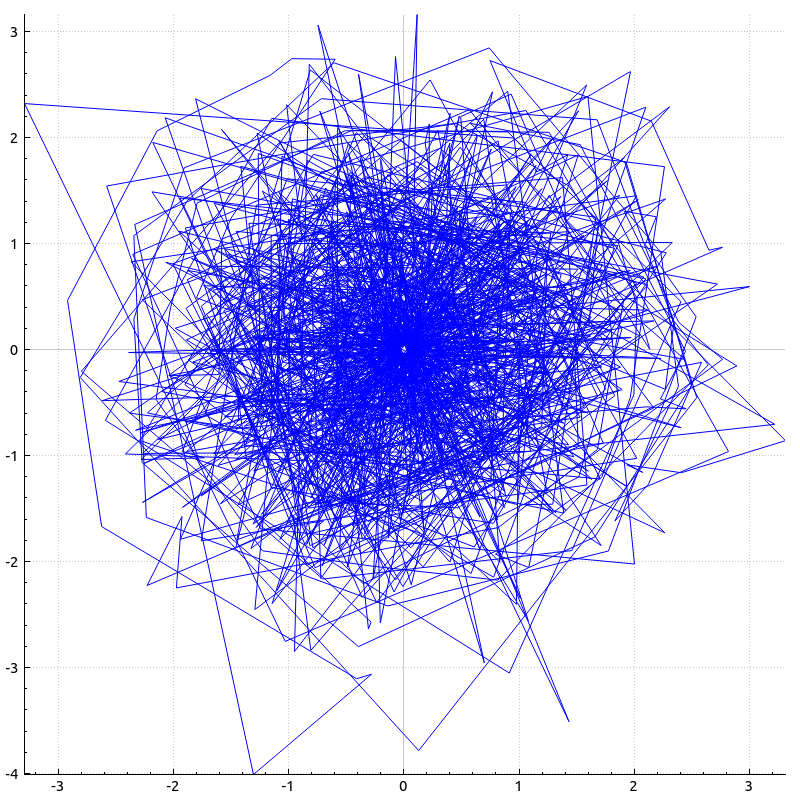
\includegraphics[width=\textwidth]{img/bps_ref_0_1}
    \caption*{$\lambda_{\text{ref}} = 10^{-1}$}
  \end{subfigure}
  \begin{subfigure}{.25\textwidth}
    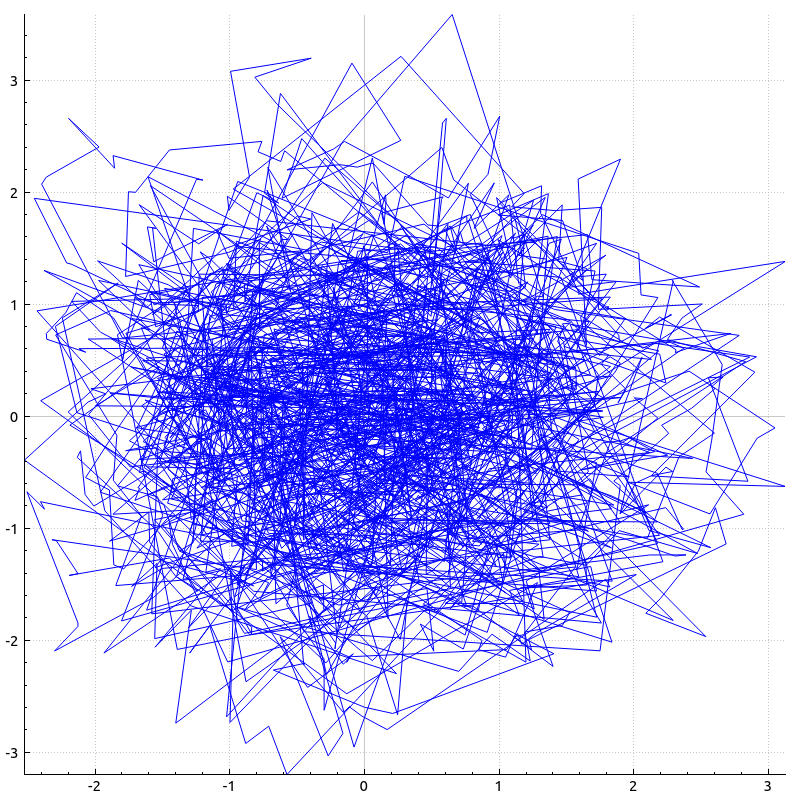
\includegraphics[width=\textwidth]{img/bps_ref_1}
    \caption*{$\lambda_{\text{ref}} = 1$}
  \end{subfigure}
  \begin{subfigure}{.25\textwidth}
    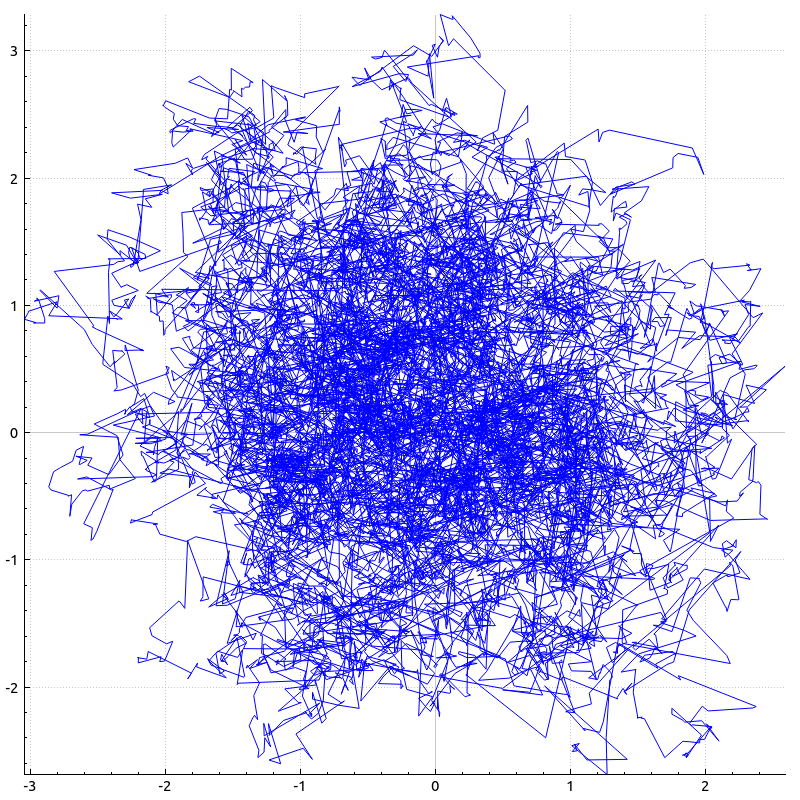
\includegraphics[width=\textwidth]{img/bps_ref_10}
    \caption*{$\lambda_{\text{ref}} = 10$}
  \end{subfigure}
  \begin{subfigure}{.25\textwidth}
    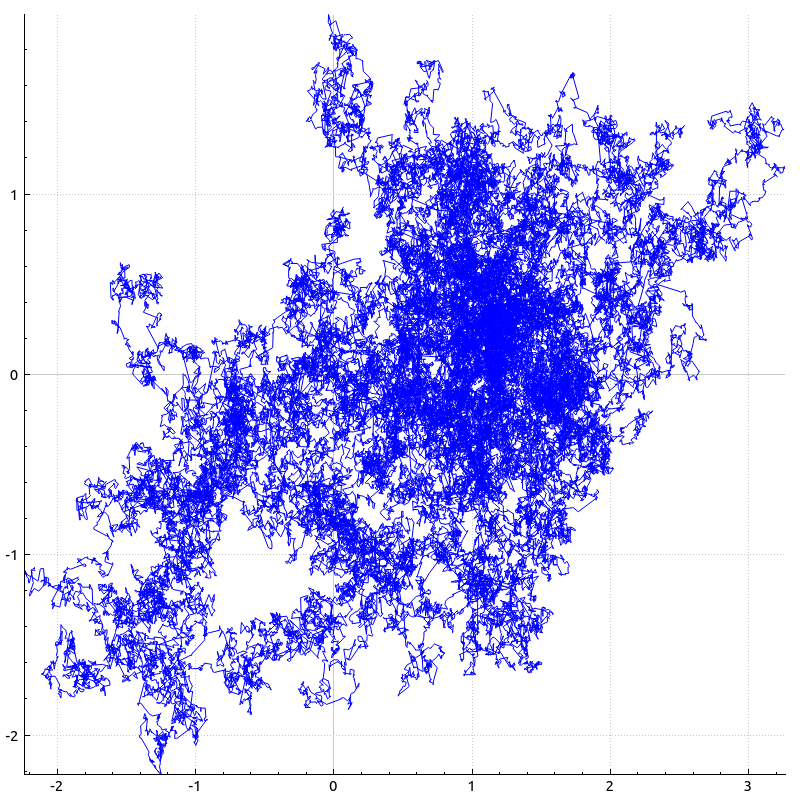
\includegraphics[width=\textwidth]{img/bps_ref_100}
    \caption*{$\lambda_{\text{ref}} = 10^{2}$}
  \end{subfigure}
  \begin{subfigure}{.25\textwidth}
    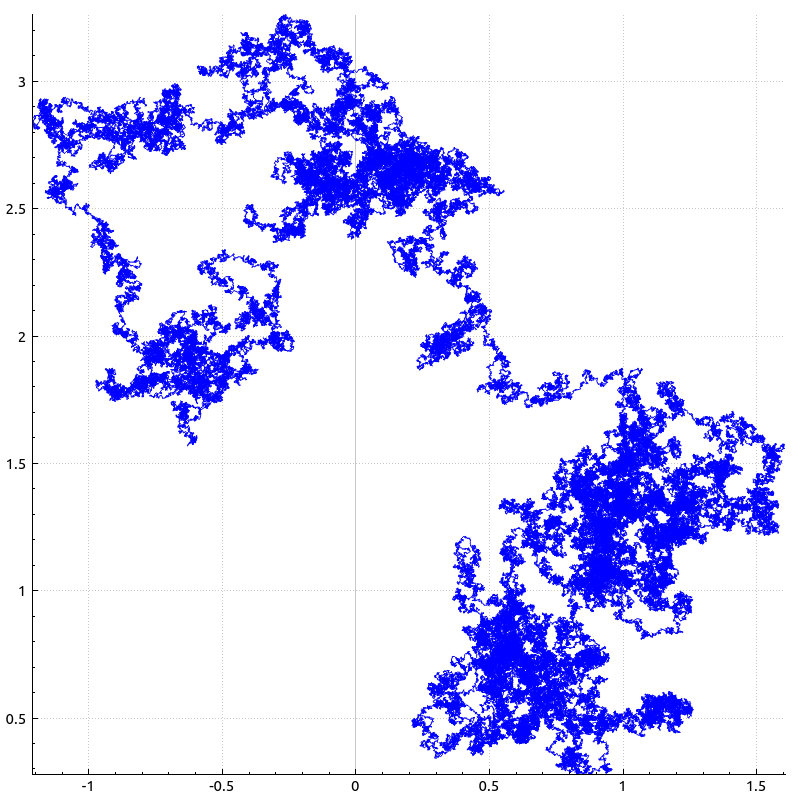
\includegraphics[width=\textwidth]{img/bps_ref_1000}
    \caption*{$\lambda_{\text{ref}} = 10^{3}$}
  \end{subfigure}

  \caption{The role of the refresh rate parameter in the Bouncy Particle Sampler.
           In each image, a trajectory path of the BPS is plotted, where
           the target distribution is 2-dimensional standard normal.
           Both too small and too large values of $\lambda_{\text{ref}}$ lead to
           difficulties in exploration of the state space. Indeed, it was shown
           in \citet{bouchard2015bouncy} that with $\lambda_{\text{ref}} = 0$ the
           resulting Markov process need not be ergodic.
           See examples/path\_plotting/ in the project's GitHub repository for
           reproducing these plots.}
  \label{image-bps-refresh-rates}
\end{figure}

\end{document}
